\chapter{Background}
\label{sec:state}

% Hier werden zwei wesentliche Aufgaben erledigt:

% 1. Der Leser muß alles beigebracht bekommen, was er zum Verständnis
% der späteren Kapitel braucht. Insbesondere sind in unserem Fach die
% Systemvoraussetzungen zu klären, die man später benutzt. Zulässig ist
% auch, daß man hier auf Tutorials oder Ähnliches verweist, die hier auf
% dem Netz zugänglich sind.

% 2. Es muß klar werden, was anderswo zu diesem Problem gearbeitet
% wird. Insbesondere sollen natürlich die Lücken der anderen klar
% werden. Warum ist die eigene Arbeit, der eigene Ansatz wichtig, um
% hier den Stand der Technik weiterzubringen? Dieses Kapitel wird von
% vielen Lesern übergangen (nicht aber vom Gutachter ;-), auch später
% bei Veröffentlichungen ist "Related Work" eine wichtige Sache.

% Viele Leser stellen dann später fest, daß sie einige der Grundlagen
% doch brauchen und blättern zurück. Deshalb ist es gut,
% Rückwärtsverweise in späteren Kapiteln zu haben, und zwar so, daß man
% die Abschnitte, auf die verwiesen wird, auch für sich lesen
% kann. Diese Kapitel kann relativ lang werden, je größer der Kontext
% der Arbeit, desto länger. Es lohnt sich auch! Den Text kann man unter
% Umständen wiederverwenden, indem man ihn als "Tutorial" zu einem
% Gebiet auch dem Netz zugänglich macht.

% Dadurch gewinnt man manchmal wertvolle Hinweise von Kollegen. Dieses
% Kapitel wird in der Regel zuerst geschrieben und ist das Einfachste
% (oder das Schwerste weil erste).

In this chapter, I will provide background information on the topics revolving
around creating a standalone \gls{tee} that uses primitives of the processor
core to isolate itself. For this, I first introduce basics about how x86
processor programming works in section~\ref{sec:state:technical}. Then we
revisit \glspl{tee} in general and how important building blocks look (c.f.
sections~\ref{sec:20:building_blocks} and~\ref{sec:state:tee}). We continue in
section~\ref{sec:20:attacks} to learn about attacks and in
section~\ref{sec:20:mitigations} before I finally summarize this chapter in
section~\ref{sec:20:summary} to highlight approaches best to my knowledge, not
employed in related work so far.

\section{Technical Background}
\label{sec:state:technical}
This chapter gives us an overview of important mechanisms used by modern CPUs.
While there are other widely used architectures, such as Arm on mobile devices,
we explore these features in the example of the x86\_64 architecture. I decided
to do so because my proof of concept implementation targets the x86\_64
architecture, more precisely Intel's implementation of the \gls{isa}.

\subsection{Privilege Levels}
\label{sec:state:technical:priv}
The x86 \gls{isa} implements the following four privilege levels:
\begin{itemize}
  \item Level 0: \gls{os} kernel
  \item Level 1 and 2: \gls{os} services
  \item Level 3: User applications
\end{itemize}
Privileges granted by the processor increase with decreasing level, which means
that level 0 implies the highest privileges and level 3 the least amount. The
processor ensures that data can only be accessed by code that runs on a
privilege level that is higher than or equal to that defined for the data. All
four levels can be used together with memory segmentation. With paging, only one
bit is used to differentiate between privileged and unprivileged
accessibility~\cite{intel_sdm}. Moreover, only level 0 grants access to all
instructions available. For example, the \textit{WRMSR}, \textit{RDMSR}, and
\textit{HLT} instructions are included in the set of instructions only available
from level 0. For the remaining parts of this thesis, when I write about
\textit{privileged software} or \textit{system software}, I am referring to
software running at level 0. Whenever I write \textit{user space software} or
\textit{application}, I refer to code running at privilege level 3.

\subsection{Operation Modes}
\label{sec:state:technical:modes}
% The x86 architecture is rooted in the Intel 8086, designed in 1978. As a 16-bit
% microprocessor design, the Intel 8086 physically can only address 64 KiB of
% memory, which was enlarged by two segment registers to allow addressing nearly 1
% MiB of memory.
One advantage of the x86 \gls{isa} is its backward compatibility that allows
modern processor to execute code written for older CPU designs. To maintain
compatibility with legacy CPUs, over the course of time additional operation
modes were introduced to the \gls{isa}. Modern CPUs allow to execute 16-bit
legacy software in \gls{g_rmode}. The \gls{g_pmode} was introduced together with
memory protection to the x86 \gls{isa}. With x86\_64 the \gls{isa} is extended
by \gls{g_lmode}~\cite{intel_sdm}. To maintain the aforementioned compatibility
to legacy software, all x86 systems start in 16-bit \gls{g_rmode}. Because of
the limitation of the address space to the first 1 MiB of memory, code that
transfers a processor from \gls{g_rmode} to any other operation mode has to
reside in the address range of 0x500 to 0x7FFFF. This address range is called
low memory and is free for usage by system software.

% introduced an operation mode called
% \gls{g_rmode}. The name  originates from the fact that the 16-bit
% design used the real location in memory for addressing. The 32-bit operation
% mode of this CPUs is called \gls{g_pmode}, because it allows addressing memory
% through virtual addresses, allowing for memory protection. All x86 processors
% boot in \gls{g_rmode} to maintain compatibility to legacy software originally
% written for 16-bit CPUs. With the 64-bit extension x86\_64, AMD introduced an
% operation mode called \gls{g_lmode} that consists of two sub-modes called
% Compatibility Mode and 64-bit mode. Compatibility mode allows 64-bit system
% software to execute legacy 32-bit software. 64-bit mode extends the \gls{isa} by
% 64-bit operands and addresses, adds eight new general purpose registers and
% additional instructions. To use \gls{g_lmode}, system software has to prepare
% the processor by enabling additional processor features and creating required
% data structures.

\subsection{System Management Mode}
\label{sec:state:technical:smm}
Contrary to the operations modes described in
section~\ref{sec:state:technical:modes}, \gls{smm} does not activate additional
processor features. Instead, it is a hardware-assisted isolation mechanism that
protects firmware code from system software. In legacy systems, firmware used
the \gls{smm} to react to special hardware events that required the firmware to
react to platform events, e.g., energy management~\cite{intel_sdm}. The
\gls{smm} code resides in a specially protected area of the main memory,
referred to as \gls{smram}. \gls{smm} executes with privileges higher than level
0, and system software cannot interfere with it. In fact, \gls{smm} can
interrupt systems software whenever necessary, not vice versa. Firmware has to
issue a \gls{smi} to enter \gls{smm}.

\subsection{Virtualization}
\label{sec:state:technical:virt}
After Popek et al., a \gls{vm} is characterized by the following
definition:
\begin{quote}
  \textit{ A virtual machine is taken to be an efficient, isolated duplicate of
    the real machine. \\
  } \mbox{ -- Popek et. al. ~\cite{popek1974formal}}
\end{quote}
To allow the duplicate to run efficiently, a special environment is created that
enables the duplicate to use the resources of the real machine. To create this
environment, a piece of software called  \gls{vmm} is used. The \gls{vmm}
controls the resources of the real machine and ensures isolation between
duplicates and the real machine. To allow the \gls{vmm} to remain in control of
the real machine, a virtual environment is configured in a way that it traps
upon special conditions. These condition are, for example, access to memory or
the execution of instruction that would influence the real machine in a way,
that the \gls{vmm} could lose control over it. In such a case, control is
transferred back to the VMM. Processor architectures have to fulfill different
conditions to be called virtualizable. In the case of x86, additional \gls{isa}
extensions allow for virtualizability~\cite {adams2006comparison}. AMD
processors implement the Secure Virtual Machine (SVM) extensions while Intel
processors implement Intel Virtualization Extensions (VT-x or
VMX)~\cite{amd_manual, intel_sdm}.
inter-processor interrupt
\subsection{Interrupts and Exceptions}
\label{sec:state:technical:interrupts}
Interrupts and Exceptions are used to call system-specific functions and respond
to special conditions in the CPU or system. Exceptions are raised by the CPU
upon executing software or detecting hardware errors. Interrupts, on the other
hand, are either the result of software interrupt instructions or signals
generated by external hardware, such as keyboard input.
% Exceptions can be
% divided into three types by their origin or if they allow to restart the causing
% instruction:
% \begin{enumerate}
%   \item Faults: Result of an error with the instruction to execute
%   \item Traps: Result of breakpoint and software interrupt instructions
%   \item Aborts: The causing instruction cannot be restarted
% \end{enumerate}
Interrupts, can be divided into two classes:
\begin{enumerate}
  \item Maskable Interrupts: Masking an interrupt means that software can
    temporarily disable them. The interrupt controller holds them back until
    interrupts are enabled again.
  \item \Gls{nmi}: Software cannot turn off \glspl{nmi}. The interrupt
    controller delivers \glspl{nmi} to the CPU unless it currently serves
    another \gls{nmi}. When the CPU executes the IRET instruction in the
    interrupt handler, the interrupt controller can deliver the next \gls{nmi}.
\end{enumerate}

The x86 \gls{isa} assigns a vector number to each interrupt or exception. Vector
numbers range from 0 to 255 in newer implementations. The CPU uses the vector
number of an interrupt as an index to locate the respective handler function in
a data structure called the \gls{idt}. The \gls{idt} resides in the main memory
and contains the address of an interrupt handler routine for each vector. System
software defines the handler routines and writes their addresses to the
\gls{idt}. Once system software defines the handler routines, it makes the
\gls{idt} active by writing its address to the \gls{idtr}. System software
cannot write directly to the \gls{idtr} but has to prepare the special memory
descriptor from which the LIDT instruction loads the \gls{idt}. After setting up
and loading the \gls{idt}, the CPU executes interrupt handlers as defined by
system software. System software can enable maskable interrupts by executing the
\textit{STI} instruction. or disable them by executing the \textit{CLI}. \\

% Over time, interrupt controllers were improved and adapted to new use cases
% similar to CPUs. In \gls{g_rmode}, the CPU falls back to using the Intel 8259 or
% a compatible programmable interrupt controller (PIC), that delivers
% interrupts to the CPU. Once the PIC delivers an interrupt to the CPU, the system
% software must serve it and signal the PIC with an \gls{eoi}, that the serving
% routine is done. \\

\begin{figure}
  \begin{center}
    \includestandalone{images/lapic.tex}
    \caption{Illustration of how \glspl{lapic} integrate in a
    multiprocessor system (Figure after~\cite{amd_manual}, p. 1075)}
    \label{fig:state:technical:lapic}
  \end{center}
\end{figure}

In modern systems, multiprocessor configurations are prevalent, and each logical
processor core has its own Advanced Programmable Interrupt Controller (APIC).
Because the APIC is CPU local, these APICs are called local APICs or
\gls{lapic}. \glspl{lapic} forward interrupts from different sources to the
respective CPU core. For example, the \gls{lapic} receives interrupts such as
\glspl{ipi} from other \glspl{lapic} and forwards legacy interrupts from the PIC
via the LINT0 pin. CPU external devices can deliver their interrupts to the
IOAPIC, which forwards them to the respective \gls{lapic}. Devices that
implement PCI version 2.2 and later do not use the IOAPIC. Instead, these
devices use Message Signaled Interrupts by directly writing to a memory-mapped
register of the \gls{lapic}. Figure~\ref{fig:state:technical:lapic} shows a
schematic view of how the \gls{lapic} of each CPU core integrates into the
system. All \gls{lapic} registers are mapped to the 4-KiB \gls{lapic} register
space starting at the address specified in the \gls{lapic} base address
register. System software can then access \gls{lapic} registers with memory
reads and writes to the APIC register space. Most interrupts require the CPU to
interact with the \gls{lapic}. Exceptions are \gls{smi}, \gls{nmi}, INIT and
STARTUP \glspl{ipi}, as well as ExtINT. These interrupts are sent forwarded
directly to the CPU by th \gls{lapic}~\cite{amd_manual, intel_sdm}. \glspl{smi},
INIT and STARTUP \glspl{ipi} are not routed through the \gls{idt}. As described
in section~\ref{sec:state:technical:smm}, a \gls{smi} invokes the \gls{smm}.
INIT \glspl{ipi} transfer the CPU into a special state that effectively halts it
until it receives a STARTUP \gls{ipi}. All other interrupts are held pending by
the processor, and the CPU is reset to an initial state. The STARTUP \gls{ipi}
causes the CPU to begin processing a bootstrap routine, whose memory address
number is placed in the Vector field.

\subsection{Caches}
\label{sec:state:technical:caches}
% Since 1980, the performance growth of memory and processors has diverged
% steadily with an ever-growing gap. Hennessy et al. note a difference in
% performance growth of factor 1,000 for a single CPU core and memory
% technologies~\cite{hennessy2011computer}. To come by this disparity, CPU a
% on-chip buffer called cache memory.\\

% With processors gaining capabilities to
% process more and more data in parallel, for example by increasing the core count
% or introducing new instructions, the demand for fast memory further grows. For
% example, from November 2023 to January 2024, the number of systems in the TOP500
% list that employed CPUs with 96 cores per socket increased from 0 to 3, with the
% former maximum number of cores per socket being 72~\cite{top500}. To hide
% latencies and bridge the gap between CPU demand and actual main memory
% bandwidth, CPUs today employ fast local on-chip memory to buffer data they
% already accessed. If they reaccess this memory item, they can use these buffers
% to speed up access. This on-chip buffer described is called cache.\\

The cache is an integral component with the purpose of speeding up memory access
and organized in a multi-level hierarchy in modern CPUs. In this hierarchy, the
lowest and the nearest to the core level, called the L1 cache, implements the
fastest access. Most modern x86 CPUs divide their L1 cache into two parts: L1D
for data and L1I for instructions. With increasing levels, caches grow in size
but tend to be slower. For example, while the L2 Cache of AMD's recent Zen4 CPUs
offers only 14 cycles of latency, the L3 cache of the same CPU has a latency of
50 cycles~\cite{zen4}.\\

When the CPU tries to access data, it first queries the fastest cache. If the
CPU can locate the data in the cache, this is called a cache hit. On a cache
hit, the CPU can profit from reduced access time and improved bandwidth. The
opposite of a cache hit is called a cache miss, after which the CPU subsequently
queries the next level in the memory hierarchy. If it finds the data needed, the
CPU loads it into the nearest cache for faster access. Caches can only store a
limited number of items, organized in cache lines. Cache lines are a copy of the
main memory, and the processor uses this copy for all of its operations unless
otherwise configured. The processor loads data in cache line size granularity
from the main memory. All of this happens transparent to software and the
processor automatically manages its cache. \\

% Caches use the principle of locality, which consists of two kinds of locality.
% The first is called spatial locality. Spatial locality describes the observation
% that if a program accesses data from the main memory, data located at nearby
% addresses are the target of future accesses with a high probability. In this
% case, without any prefetching, the CPU tries to guess the size of the loaded
% structure to load parts missing in the cache in advance. If the CPU then
% accesses the neighbor of the first data, it already resides in the cache,
% lowering the latency. The second principle is temporal locality, which states
% that a program soon reuses memory references with a high probability. The CPU
% can, therefore, gain performance by storing recently used data in the cache for
% reuse.\\

With cache lines being copies of main memory items, and the possibility of
multiple copies of the same item existing in multiple caches at the same time,
the need for keeping them consistent arises. For this, different strategies for
writing data back to main memory exist:
\begin{itemize}
  \item \textbf{write-back}: Data modified in the cache is stored and written
    back to the main memory later. Cache coherency protocols are required to
    allow multiple devices to access the same memory range.
  \item \textbf{write-through}: The changes in the cache are instantly written
    to the main memory. These writes can slow down program execution because of
    costly main memory writes, but ensure consistency with system memory and
    cache content. This type is relevant for devices that access system memory
    but do not access CPU cache.
  \item \textbf{cache-disable}: The CPU cache is disabled, and the CPU
    performs all memory operations using the main memory.
\end{itemize}
% Legacy x86 software controls cache settings by setting or clearing configuration
% bits in the control register CR0. In a system employing modern x86\_64
% processors, systems software can set the caching strategy on page granularity
% (c.f. Chapter~\ref{sec:state:technical:paging}) by setting and clearing the
% respective bits in the page table entries. These settings are used in
% conjunction with values of the Memory Type Range Registers (MTTR) and Page
% Attribute Table (PAT) to calculate the effective caching strategy for a physical
% address.

Legacy x86 software has different ways of managing the cache settings than
modern \gls{os}. In modern \gls{os}es that use paging, the processor ignores the
write-through setting of CR0 and uses the page-level settings
instead~\cite{amd_manual}. The default in x86\_64 processors is to use a
write-back strategy.

\subsection{Cache coherence protocols}
\label{sec:state:technical:caches_protocol}
%An interesting difference in the x86\_64 implementation of Intel and AMD
%processors are the cache coherency and inclusion policies.
%AMD processors useMOESI as a cache coherency protocol~\cite{amd_manual}.
Intel processors
%,on the other hand,
use MESIF as a coherency protocol to maintain consistency of the caches among
different CPUs~\cite{thomadakis2011architecture}.
%MOESI and
MESIF is an extension of the MESI protocol, introducing the additional
\textit{Forward} state respectively.

The meaning of the states in the MESIF protocols are as follows:
\begin{itemize}
  \item \textbf{Modified}: The copy in the processor's cache is the most
    recent and modified. The copy in the main memory needs to be updated.
    Other processors in the system might maintain stale copies.
  \item \textbf{Shared}:  The copy is the most recent and correct copy of the
    data. Other processors may hold copies, too. Main memory holds the
    most recent and correct copy, too.
  \item \textbf{Exclusive}: The processor's and the main memory's copy are the
    most recent and correct copies. No other processor holds a copy.
  \item \textbf{Invalid}: The cache line is invalid and needs to be replaced by
    a valid copy from main memory or other CPU's caches before it can be used.
  \item \textbf{Forward}: Only one processor can hold a cache line in this
    state. Other processors might hold a correct copy of the cache line in
    shared state. The owning core responds to requests. The cache line is clear,
    so no writeback is required before discarding the line.
\end{itemize}

\begin{figure}
  \begin{center}
    \includestandalone{images/mesi.tex}
    \caption{MESI state transition of a cache line resulting from a (remote) activity (after~\cite{mckenney2010memory}, p. 4)}
    \label{fig:state:technical:mesi}
  \end{center}
\end{figure}

All cache lines are tracked to be in one of the states.
Figure~\ref{fig:state:technical:mesi} shows transitions of MESI states of a
cache line as a result from a core's own or another core's remote
access~\cite{mckenney2010memory}. The \textit{forward} state is essentially
equal to the \textit{shared} state when it comes to state
transitions~\cite{hay2012mesif}. It was created as an optimization to the MESI
protocol and reduces overhead in multi node
architectures~\cite{goodman2004mesif}. Important for my use case are the
following state transitions:

\paragraph{Foward from/to Shared}
Processor $0$ has the \textit{forward} copy of a cache line. Processor $1$
acquires a copy to read from processor $0$. Processor $1$ is the most recent
requester of the item and forwards it if any other processor requests a copy. It
holds the line in \textit{forward} state. Processor $0$ does not answer to
requests anymore, it now holds the cache line in the \textit{shared} state.

\paragraph{Exclusive to Shared}
Processor $0$ has the \textit{exclusive} copy of a cache line. Processor $1$
acquires a copy to read. In this case, the state of the line in processor $0$'s
cache changes from \textit{exclusive} to \textit{shared} to reflect that other
cores use the line.

\paragraph{Shared to Modified/Exclusive/Invalid}
Processor $0$ and processor $1$ both have the same data item in their local
caches. The state of both copies of the cache lines is \textit{shared}. Before
processor $0$ writes to the cache line it triggers the \textit{invalidation} of
the line in processor $1$'s cache. Upon receiving the acknowledgement of
\textit{invalidation} from processor $1$'s cache line, processor $0$ changes the
state of its cache line from \textit{shared} to \textit{exclusive}. At this
point the cache line is clean and matches the copy in the main memory.
Transferring a cache line to \textit{exclusive} can be done in preparation to an
anticipated write. After writing to the cache line, its state is changed to
\textit{modified}. If processor $0$ performs an atomic read-write operation it
will change its copy directly from \textit{shared} to \textit{modified}. The
state of the cache line in processor $1$'s cache is now \textit{invalid}.

Processors write back their data to the main memory once a cache line is evicted
or when other processors request the same data item. If another processor
requests the data item, then the owning processor will make the item available
via inter-cache transfers or through a writeback.

\subsection{Cache Inclusion Policies}
\label{sec:state:technical:caches_inclusivity}
On all current x86\_64 multicore CPUs, the \gls{llc} is shared among all cores
for synchronization and uses one of the coherency protocols. Older multicore
CPUs produced by Intel use an inclusive \gls{llc}, while more recent ones use a
non-inclusive \gls{llc}~\cite{intel_optimization, raptorlake_spec_sheet}. An
inclusive cache describes a cache containing the same content as lower levels
and vice versa. A line evicted, for example, in the \gls{llc}, is also evicted
in the lower levels. If an item is modified in a lower cache level, the changes
are automatically propagated to the higher inclusive cache
level~\cite{backes2019impact}. The opposite of an inclusive cache is an
exclusive cache design, as used by recent AMD CPUs~\cite{amd_z4_optimization}.
Exclusive caches do not replicate data in upper levels. Instead, the exclusive
cache level serves as a victim cache of the lower levels. Non-inclusive caches
can contain items of the lower levels, but inclusion is not enforced. This
means, if a line is evicted from higher levels its eviction is not enforced in
the lower levels~\cite{backes2019impact}.

\subsection{Hardware Performance Monitoring Counters}
\label{sec:state:technical:hpc}
\glspl{pmc} are registers that increment on the occurrence of predefined
microarchitectural events. The x86\_64 \gls{isa} specifies four freely
programmable general purpose \glspl{pmc}~\cite{amd_manual}. Concrete processor
implementations can offer additional counters. Similarly, the \gls{isa}
specifies architectural events that must be present in every processor
implementing x86\_64. Additional events are vendor and implementation-specific.
The four general purpose counters can be programmed to count any event supported
by the respective processor implementation. Vendors of x86 CPUs publish what
processor supports what additional events in their manuals. Moreover, a CPU
reports what events it supports in the result of the \gls{g_cpuid} instruction.
\\

In x86 hardware, performance counters are implemented by a set of two
\glspl{msr} per counter. One \gls{msr} can be programmed by system software with
the event to measure, while a second \gls{msr} counts the occurrence of the
respective event. Reading \glspl{pmc} can be done with the privileged RDMSR
instruction or from user space with the RDPMC instruction. In this way, a
program can poll the values of counters. The system software can also program a
threshold for a \gls{pmi}. Once the \gls{pmc} values exceed the threshold, the
\gls{pmi} is triggered, offering an alternative to expensive polling
techniques.\\

When using hardware \gls{pmc}, one must use the proper technique adopted to the
environment in which to obtain the counter values. Das et al. found in a
comprehensive survey that noise from the system is often present, e.g. context
switches influence the values of performance counters~\cite{das_sok_2019}.
Moreover, some counter events are over-counted while the CPU can undercount
others~\cite{weaver_non-determinism_2013}. It is therefore important to check
the right conditions for using hardware counters and verify that they work
correctly.

\subsection{Paging}
\label{sec:state:technical:paging}
% With the evolution of computer systems not strictly processing data in a batched
% manner anymore but instead allowing for multiple applications to run
% concurrently, a need for complex memory management arose. For example, system
% software must ensure that two applications programmed to use the same memory
% addresses do not influence each other. Segmentation is a legacy technique used
% in x86 systems to solve this problem. Segmentation allows the construction of
% address spaces that allow transparent translation of application addresses
% within an address space dedicated to the application. However, if applications
% do not entirely fit into memory, system software must perform expensive swapping
% operations between main and disk memory. In this swapping operation, programmers
% either need to split up their application into parts that must reside in the
% main memory simultaneously, or system software must swap the complete
% application.\\

% A solution to this is virtual memory implemented through
% paging~\cite{tanenbaum2015modern}.

The preferred way to manage memory in modern x86\_64 system is a technique
called paging. Paging splits the virtual address space into small, evenly
sized-parts called pages. The main memory is split into parts of the same size,
called page frames, by which each page can be backed.
% By splitting the address
% space into pages, system software can now perform swapping more fine-grained. If
% an application accesses a page not backed by a frame, hardware emits a fault,
% and system software can take the necessary steps to load it into physical
% memory. On the other hand, applications are now implicitly split into parts,
% allowing system software to only swap out parts of running applications.
% Additionally, paging allows applications to theoretically use the whole address
% space, with system software to decide what virtual address is currently backed
% by what physical page frame through its mapping function. This allows system
% software even to map a single physical page frame to the address spaces of two
% applications simultaneously, for example, if both applications use the same
% shared library. Knowing in detail how paging work on x86\_64 hardware will help
% understand content of later chapters.\\

% \begin{figure}
%   \begin{center}
%     \includestandalone{images/paging.tex}
%     \caption{Illustration of Virtual Address Translation with 4 Levels of Page Tables (after~\cite{amd_manual}, p. 597)}
%     \label{fig:state:technical:paging}
%   \end{center}
% \end{figure}
Hardware uses page tables that are hierarchically organized for the translation
of virtual to physical addresses. Each page table forms a level in the table
hierarchy and is the size of one page, storing references (addresses) to the
next lower level. The last page table in this hierarchy stores the address of
the physical page frame.
% By default, x86\_64 uses pages of size 4 KiB. Because
% x86\_64 uses 64-bit addresses, each 4 KiB sized page table can store 512
% entries. Figure~\ref{fig:state:technical:paging} shows the page translation of a
% virtual 64-bit address in x86\_64 with a page table hierarchy of four levels and
% a page size of 4 KiB. A virtual 64-bit address consists thereby of indices in
% the respective page tables to find the address as an entry in the lowest-level
% page table. Each page table in the hierarchy is referenced by its physical
% address.\\

% A virtual address for x86\_64 4-level paging with 4 KiB page size is divided
% into a 12-bit field used as an index in the page frame and four 9-bit fields,
% which the hardware uses as an index to access the content of the respective page
% level. The remaining address bits are sign extensions of bit 52, forming a
% canonical address. The hardware must perform a page table walk to resolve the
% virtual address.
% For the first step of a page table walk, the processor locates the address of
% the first page table, in this case, the PML4 table. The address of the PML4 is
% written by system software to CR3 after it created the page table. All page
% tables are aligned to 4 KiB, which leads to a value of 0 for the 12 least
% significant bits. Depending on the configuration, these 12 bits in CR3 are
% either used to determine the memory type of the PML4 or to store process-context
% identifiers.
To access the first table of the hierarchy, the CPU reads its physical address
from CR3.\\
% It uses the 9-bit index of the PML4 offset field in the virtual
% address to find the Page-Map-Level 4 entry containing the address of the next
% page table, the Page-Directory-Pointer table. The CPU accesses this table and
% all successor tables similarly until it locates the physical page. To access the
% data that belongs to the virtual address, the CPU uses the last 12 bits of the
% virtual address as an index to access the respective byte in the page frame. \\

% As the page table walk is expensive, the \gls{mmu} automatically stores the
% translated addresses in a cache called \gls{tlb}. System software has to manage
% page tables and \glspl{tlb} for each CPU independently. Furthermore, system
% software must maintain consistency between page tables and each \gls{tlb} by
% invalidating individual entries or the entire \gls{tlb}. If system software
% invalidates an entry, the CPU has to complete a page walk for this virtual
% address, upon which the \gls{mmu} updates the \gls{tlb}. Similar to other
% caches, filling entries in the \gls{tlb} works transparent to software. System
% software can use the INVLPG instruction to explicitly invalidate the \gls{tlb}.

\begin{figure}
  \begin{center}
    \includestandalone{images/pte_rights.tex}
    \caption{Layout of the 12 least significant bits in a page table entry (after~\cite{amd_manual}, p. 592)}
    \label{fig:state:technical:paging_rights}
  \end{center}
\end{figure}
The 12 least significant bits of each page table entry are used for management
properties, such as access rights management.
Figure~\ref{fig:state:technical:paging_rights} shows the layout of the 12 least
significant bits of a page table entry. The present bit is another property
stored in the 12 least significant bits of a page table's entry. It indicates if
the page the respective entry points to was initialized and loaded to the page
table. If this bit is clear, the CPU generates a \gls{pf} exception and expects
system software to load the respective entry. The CPU also generates a \gls{pf}
if software violates access rights. A second bit important for this thesis is
the Page-Level Cache Disable (PCD) bit. If the PCD bit is set, the CPU cannot
cache the respective page. Bit 3 (PWT) controls page-level write-through. If
system software sets this bit, the page table has a write-through caching
policy.

\section{Chain of Trust}
\label{sec:20:chain_of_trust}
Signatures of real humans differ because humans do not work entirely
deterministic. The process of forging signatures of other humans requires
dictations and practice by the forger because the human factor introduces
entropy to the process of signing. On the contrary, computers are built to work
deterministically. If the same input data is processed the same way, computers
working as intended by humans produce the same output. It is, therefore, that
authentication in the digital realm is implemented through cryptography and the
knowledge of secrets. Communication involves at least two parties, which we want
to call Alice and Bob in the following example.\\

When referring to cryptographic algorithms, a secret is called a key, and based
on the kind of keys used, we can differentiate between two kinds of
cryptographic algorithms. In symmetric algorithms, the same key is used for
encryption and decryption. Alice and Bob share thus the same secret. In
asymmetric algorithms, each of Alice and Bob maintain their secrets. These keys
have a public and a private part, respectively. Alice uses the public part of
Bob's key when they want to encrypt a message for Bob, and only Bob's private
key can decrypt a message in this way.\\

Digital signatures use asymmetric cryptography. Given that Alice wants to sign a
message so that Bob can verify that Alice is the sender, both proceed as follows
to fulfill their goal. First, Alice creates a pair of keys, a public and a
private one. Alice uses their private key to sign a message and distributes
their public key so others can use it to verify Alice's signature. To create
their signature, Alice first generates a pair of keys. Alice then published
their public key to make it available to Bob. When sending a message to Bob,
Alice uses a signing function that takes the message and the private key as
input and produces a signature, which Alice sends along the message to Bob.
Knowing Alice's public key, Bob can now check the validity of the signature with
the help of a signature validation function. This function takes the message,
the signature, and Alice's public key as input and generates the answer to
whether the message was signed with the signature.\\

Another problem arises when the network increases and Bob does not have the
chance to receive Alice's key in person. To prevent man-in-the-middle attacks,
Bob must ensure that the key they received over a network originates from Alice
and not from a malicious entity. The attack surface increases with the number of
different entities Bob wants to communicate with, as Bob needs to verify the
keys of each of their communication partner. A third party, the \gls{ca}, that
Bob trusts, can help with this. The \gls{ca}'s task is to pledge to Bob that a
certified key belongs to Alice or any other chosen entity and not a potentially
malicious third party. Bob trusts the \gls{ca} to do the keys' background check
and only deliver certificates of trusted identities. Alice first registers their
key with the \gls{ca}. The \gls{ca} own a pair of private and public keys too.
It uses these keys to cryptographically bind Alice's public key to their
identity. With this certificate, Bob can validate that a public key belongs to
Alice by validating the certificate with the \glspl{ca} public key. Alice now
delivers their public key and the certificate issued by the \gls{ca} to prove
that the key belongs to them. As long as the \gls{ca} is not malicious, Bob can
detect man-in-the-middle attacks if any malicious entity ships a key not
belonging to Alice. While all participants can create certificates for their key
with a dedicated key pair, such self-signed certificates could allow
man-in-the-middle attacks again. Hence, a trusted third party creates the
certificates.\\

\begin{figure}
    \begin{center}
        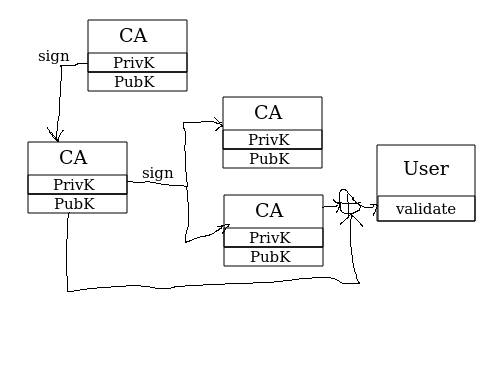
\includegraphics[width=.6\textwidth]{images/chain_of_trust_placeholder.png}
        \caption{Certifications in a chain of trust}
        \label{fig:state:technical:chain_of_trust}
    \end{center}
\end{figure}
\todo{This is a placeholder}

Because the single \gls{ca} is trusted by all participants in the network,
compromising it would mean control over all the communication in the network.
The solution to this is distributed trust. Multiple \gls{ca}'s can exist in a
network and compete with each other on the reputation gained from
users.\cite{perlman1999overview} Such a \gls{pki} is used in many network
technologies, such as HTTPS, that use the X.509 standard. Next to leaf
certificates issued to Alice and Bob, a \gls{ca} can also issue certificates on
keys that allow other entities to issue certificates and act as an \gls{ica},
creating a chain of certificates.
Figure~\ref{fig:state:technical:chain_of_trust} shows such a chain of
certificates. If Bob now wants to establish trust in the certificate provided by
Alice, they must first decide if they trust the \gls{ica}. The first step is to
verify that Alice's certificate was issued by the \gls{ica}. In the next step,
Bob needs to check all succeeding certificates until they reach the root
\gls{ca} by validating the \glspl{ica} respective certificates with the public
key of their issuer. In this way, Bob builds a chain of trust by verifying the
validity of the chain of certificates and deciding to trust the root \gls{ca}.
In the following section, we will see that such trust chains allow the
implementation of software attestation schemes.

\subsection{Remote attestation}
\label{sec:20:remote_attestation}
Remote attestation proves claims about a target
by delivering evidence to an appraiser over a network that supports these
claims. Before I further proceed to explain remote attestation, I want to
define the following terms similar to Coker et. al.\cite{coker_principles_2011}
\begin{itemize}
    \item \textbf{Appraiser}: Member of a network. Makes decisions about other
          parties on the base of delivered evidence.
    \item \textbf{Target}: Member of a network. Party about which properties the
          appraiser makes decisions.
    \item \textbf{Attestation}: Action of making claims about the target and
          delivering supportive evidence.
    \item \textbf{Measurement}: Collect evidence through direct and local
          observation
    \item \textbf{Attestation protocol}: Cryptographic protocol transmitting
          evidence about the claim. Trusted by appraiser
\end{itemize}

The appraiser and the target both follow orthogonal goals. While the appraiser
ideally wants to get as much information as possible about the target, the
target wants to preserve its privacy as well as possible and, therefore, conceal
as much information as possible. Both goals can be realized by employing a
trusted third party local to the target who can measure the target. This
third-party party then sends a signed report of the evidence on behalf of the
target. This report can contain the full raw measurement result, a reduced
variant, or a complete measurement substitute. For example, the reduced
measurement could be from a hash of the raw data. The substitute could be a
signature associated with the trusted third party that verifies that the target
fulfills the claims.

\subsection{Hardware Root of Trust}
\label{sec:20:hardware_root_of_trust}
A root of trust is defined by the Trusted Computing Group as follows:
\begin{quote}
    \textit{ A minimal set of system elements that have to be trusted because
        misbehavior is not detectable. \\
    } \mbox{ -- Trusted Computing Group\cite{tpm_architecture}}
\end{quote}

The Trusted Computing Group specifies that a hardware root of trust must be
available to enable remote attestation in a confidential computing
environment.\cite{tpm_architecture} A hardware root of trust is a device in a
computer system that the system can not manipulate. Moreover, it implements
security functionality such as encryption and random number generation. While
misbehavior is impossible to detect, hardware manufacturers can verify that
their devices work as intended by providing certificates. These certificates can
be embedded into the device with the help of tamper-resistant memory, such as
ROM or eFuses. A user can then check the validity of a certificate by consulting
the respective manufacturer's service. \\

Hardware roots of trust are necessary because system software could tamper with
software or memory to manipulate a possible software solution. The following
sections we review the most widely spread solutions to the hardware root of
trust. These implementations rely on dedicated hardware modules such as add-in
cards or unique, secure operation modes in CPU hardware. \\

\section{Trusted Execution Environments}
\label{sec:state:tee}

GlobalPlatform first used the term trusted execution environment to define a
solution for mobile trusted computing solutions.\cite{globaltee} Since then,
many definitions inconsistent and unspecific definitions have been published for
TEEs until the first precise definition was proposed by Sabt
et.al.\cite{sabt2015trusted}. They define the TEE in the following way:
\begin{quote}
    \textit{Trusted Execution Environment (TEE) is a tamper-resistant processing
        environment that runs on a separation kernel. It guarantees the authenticity of
        the executed code, the integrity of the runtime states (e.g., CPU registers,
        memory, and sensitive I/O), and the confidentiality of its code, data, and
        runtime states are stored on persistent memory. In addition, it shall be able
        to provide a remote attestation that proves its trustworthiness for third
        parties. The content of TEE is not static; it can be securely updated. The TEE
        resists all software attacks as well as physical attacks performed on the
        system's main memory. Attacks performed by exploiting backdoor security flaws
        are not possible. \\
    } \mbox{ -- Sabt et al.\cite{sabt2015trusted}}
\end{quote}

The first half of the definition describes a secure execution environment. A
secure execution environment can protect the integrity, authenticity, and
confidentiality of the application hosted by the SEE. Malicious privileged
software is thus neither able to modify the code, tamper with the runtime state,
nor observe code and data through the runtime. Contrary to TEEs, a SEE cannot
prove these claims against an appraiser, lest a third party outside the system.
This is because it does not require a root of trust to present in the system. To
prove its trustworthiness, TEEs employ remote attestation, which is the second
important aspect of the definition.\\

Trusted execution environment consists of several building blocks. The first
building block Sabt et al. propose is a secure boot. This building block allows
TEEs are used to verify that only a specific code of a particular state is
loaded. For a secure boot, a chain of trust is formed by verifying each
component's state. To generalize the secure boot requirement, a TEE must be
capable of verifying what code it loads to the environment. The second building
block is secure scheduling. Task executing in the TEE should not be able to
disrupt the main OS. Moreover, a TEE should implement means to allow
communication between the insecure world outside the TEE and the application
executing inside of it. Secure storage is one more building block. It allows the
application in the TEE to store data in a confidentiality, integrity, and
freshness-conserving way. Trusted I/O paths secure the communication between a
TEE and its users.

\subsection{TPM}
\label{sec:20:tpm}
\todo{A lot of passive to fix here}
The \gls{tpm} is a low-cost cryptographical coprocessor that offers different
cryptographic functions, such as hash functions, asymmetric and symmetric
encryption and decryption functions, asymmetric signing and verification
functions, and key generation functions. Implementations of the \gls{tpm} follow
different versions of specifications created and managed by the \gls{tcg}
consortium.\cite{tpm_architecture} The \gls{tpm} is specified by the Trusted
Computing Group as a system component with a state separate from the host system
on which it reports. The host system cannot directly manipulate the state of the
\gls{tpm} but has to use a defined interface to interact with the \gls{tpm}. To
separate the state between the host system and the \gls{tpm}, the \gls{tpm} is
implemented using dedicated hardware, such as a processor, RAM, ROM, and Flash
memory, all physically protected from the host system. Other physical separation
means can be used to implement \gls{tpm} services, such as unique processor
modes with dedicated memory access rights.\\

The most recent version of the \gls{tpm} specification is 2.0. The first
widespread family of \glspl{tpm} followed specification version 1.2, which was
implemented on modules shipped with personal computers beginning from the year
2005.\cite{arthur2015practical} One major drawback of version 1.2 was the
hard-coded usage of SHA-1 as a hashing algorithm. SHA-1 was first broken in 2005
by Wang et al.\cite{wang2005collision}. In 2011, NIST deprecated SHA-1 because
of security concerns.\cite{nist-sha1} \gls{tpm} 1.2 is constrained with respect
to its data structures to use either RSA or SHA-1\cite{tpm_architecture}
Therefore, when designing \gls{tpm} 2.0, the \gls{tcg} decided to leave the
exact algorithms specific \glspl{tpm} support open for their implementation.
Instead, the specification mandates a \gls{tpm} of version 2.0 to implement at
least one symmetric hashing, one symmetric encryption, and one asymmetric
encryption and signing algorithm. \\

In x86 systems, \gls{tpm} 2.0 is widely spread today and one of Windows 11s
system requirements. Often, \gls{tpm} is not implemented as a dedicated hardware
module but as firmware \gls{tpm}. The firmware \gls{tpm} is part of the Intel
Platform Trust Technology (Intel PTT) on Intel platforms. AMD platforms use an
implementation called fTPM, which is integrated within the platform security
processor.\cite{pirker2024brief} \\

While manufacturing, a vendor burns a \gls{ek} together with a certificate in
the \gls{tpm}. The \gls{ek} can be used to identify the \gls{tpm}, and the
certificate can be used to prove that the \gls{tpm} is genuine with the help of
the vendor's public key. Moreover, the \gls{tpm} uses the \gls{ek} as an input
to its key derivation functions. With the help of these key derivation
functions, a \gls{tpm} can generate keys for other applications such as
attestation, hashing, and signing. It never uses the \gls{ek} directly to
prevent leaking it in any form. A built-in entropy collector enables the
\gls{tpm} to generate random numbers. The \gls{tpm} uses hash functions to
generate a digest of input. Next to its cryptographic properties, the advantage
of a hash function is the output's constant length independent of the input's
length. Thus, the buffer only needs to be large enough to hold the result of the
digest. Message digests are used to store data outside of the \gls{tpm} or
generate certificates of values. The \gls{tpm} uses HMACs when storing data
outside of it. HMACs allow verifying that this data was not altered and
originates from a certain entity with the signing key.\\

The \gls{tcg} specifies two roots of trust for a trusted system. Two of them can
be implemented by the \gls{tpm}. The first is the root of trust for storage. The
\gls{tpm} implements memory that is shielded from the rest of the system, and
that can only be accessed by the \gls{tpm}. The second root of trust is the root
of trust for reporting. With its signing ability, the \gls{tpm} can attest to
values stored in its memory and create certificates for a measurement chain. The
third root of trust is the root of trust for measurement. This root is formed by
the CPU that measures on behalf of the system software or firmware. The
specification describes a core root of trust for measurement as the first
instructions executed in a new chain of trust, typically the firmware. In other
words, the core root of trust is trusted software that is believed to perform
the first measurement of the system correctly.\\

Software that performs the measurements instructs the \gls{tpm} to store its
result in \gls{pcr}. \glspl{pcr} are special registers of the \gls{tpm} that only
allow the \texttt{extend} operation and only reset when resetting the system.
The \texttt{extend} operation takes the current value of the \gls{pcr} and a new
value as input, concatenates both values, and processes the result with the help
of a hash function to create a digest that reflects the current system state.
The \gls{tpm} can assist in creating a chain of trust
(see~\ref{sec:20:chain_of_trust}) with the help of \glspl{pcr}. An example of how
to use the \gls{tpm} to build up a chain of trust is given by Arthur et
al.\cite{arthur2015practical} The system software can extend a certain \gls{pcr}
for each state before transferring control to the next application. The
application can then check the respective \gls{pcr} to contain a known good
value, indicating the platform was in a known good state before the application
was launched. If so, it can continue operation. If not, the application might
terminate. The measurement can also contain data about the application to be
launched to make sure that the application's integrity is not hurt. Remote
parties can use the \gls{tpm} attestation function to determine whether a system
was in a known good state at some time. For this, the \gls{tpm} offers the
possibility to sign the content of one or more \glspl{pcr}, producing a quote.
The remote party receives the quote, the public key, and the message contents.
The remote party can validate the certificate by executing the signature
validation function. With the public key of the \gls{tpm}, a remote party can
verify that the \gls{tpm} is genuine, and the vendor pledged to do so.
\todo{Do we need information on how system software interacts with the TPM?}

\subsection{Intel SGX}
\label{sec:20:sgx}
\todo{A lot of passive to fix here}
Intel SGX is an extension in x86\_64 processors manufactured by Intel, that
allows the creation of trusted execution environments. Intel first shipped SGX
in 2015, with processors implementing the Skylake microarchitecture. While
server-grade CPUs are still implementing SGX, Intel marked SGX was deprecated in
2021 in consumer-grade CPUs, beginning from CPUs implementing the Rocket Lake
microarchitecture. Costan et al. did an extensive study of SGX in 2016 and
documented in detail how SGX works and what it's security properties
are.\cite{costan2016intel} \\

Features of SGX include the creation of enclaves. Enclaves are especially
access-protected and encrypted system memory regions, with SGX preventing direct
memory access. In the creation process, memory pages are added to the enclave
page cache (EPC) and assigned to the enclave. Once assigned to an enclave, SGX
protects the memory page from unprivileged access, which includes all access
attempts not originating from the memory-owning enclave. After the system
software adds all pages to the enclave, it is marked as initialized. For the
initialization process, system software uses privileged instructions. After the
enclave is marked initialized, no more pages can be added to the EPC, and
interaction with the enclave is only allowed by using dedicated instructions
available only in user space. The EPC is similar to an inverted page table,
which purpose is to protect an enclaves security by ensuring the correctness of
the allocation process. SGX would, for example, refuse operation if it detects
that the same page frame was used for two different enclaves.\\

The enclave code runs at the permission level of
the application from which the enclave was called. Intel equips each CPU with
unique cryptographic keys that the CPU uses to encrypt code and data placed in
the EPC. These keys reside in memory made of electronic fuses that can not be
reprogrammed. Intel programs this memory in the factory process by burning some
of the fuses. Applications using SGX services do not necessarily need to run as
a whole in an SGX enclave. Because of restrictions on the size of the enclave's
memory, only parts of the data were handed to enclaves. Again, communications
between the enclave and user applications use special CPU instructions. In cases
where applications are split into parts residing in and outside of the enclave,
an application might want to verify the identity before sharing secrets. For
this, SGX implements local attestation.\\

As mentioned, SGX implements processor instructions dedicated to managing and
interacting with enclaves. Furthermore, SGX implementations create at least a
Launch Enclave signed by Intel. Third party enclaves that are not signed by
Intel require the Launch Enclave for successful initialization. It is necessary
in all cases when SGX is used.\\

An attesting enclave can verify its identity with another enclave in the same
system by generating a report. The attesting enclave calls the \textbf{ERPEORT}
instruction to generate this report. As a result, the CPU measures the attesting
enclave and generates a report that contains the measurement, the enclave's
identity, and a message provided by the enclave. The attesting enclave then
ships the generated report to another enclave for local attestation.
\begin{center}
    \begin{figure}
        \centering
        \includestandalone{images/sgx_attestation.tex}
        \caption{Software Attestation Scheme of SGX}
        \label{fig:state:tee:sgx_attestation}
    \end{figure}
\end{center}
Figure~\ref{fig:state:tee:sgx_attestation} shows the remote attestation scheme
implemented by Intel SGX. It extends the local attestation scheme so that a
third party not part of the system can verify the identity of an enclave. The
quoting enclave serves as a root of trust in this process. It is a unique
enclave provided by Intel that has access to the CPUs infused keys and can thus
act as a trust anchor. Upon receiving a report from another enclave, the quoting
enclave verifies said report and signs it. A remote third party can then check
the quoting enclave's signature to verify the correctness of the report..

\subsection{Confidential Virtual Machine Extensions}
\label{section:20:confidential_vms}
The goal of confidential Virtual machines is to protect the entire \gls{vm} from
the influence of a malicious hypervisor or other privileged software. Intel and
AMD offer individual \gls{isa} extensions for their processors to host
confidential Virtual Machines. Intel calls its solution Intel TDX, while AMDs
solution is called AMD SEV-SNP.\cite{tdx_whitepaper,kaplan_amd_2020} Both
solutions use the same fundamental building blocks to achieve the goals of
confidential \gls{vm}s. Misano et al. did a extensive comparison of both
technologies.\cite{misono_confidential_2024} Intel uses the SGX module for its
implementation. Additionally, to interact with a confidential \gls{vm}, the CPU
must be in the dedicated CPU operation mode called SEAM mode. Memory access is
only allowed in SEAM mode to protect confidential \gls{vm}s. Once in SEAM mode,
the CPU uses its Virtual Machine Extensions (VMX) capabilities to host and
interact with the \gls{vm}. For cryptographical features, such as signing and
key generation, Intel processors utilize the Intel Management Engine. The Intel
management Engine is a coprocessor located in the CPU package with special
firmware and a separate OS that is isolated from the remaining parts of the
system\\

For \gls{sev}, AMD uses the already implemented SEV capabilities and its
extensions. In its initial version SEV encrypts the memory of a virtual machine
with a dedicated key per virtual machine. SEV-ES extends the feature set by
additionally encrypting the system state, e.g. processor register, too. With the
most recent version, AMD introduced a feature called nested paging, which
manages an inverted page table similar to SGX to prevent attacks targeting the
\gls{vm}s page tables.\\

Unlike Intel's implementation, AMD processors do not utilize a dedicated CPU
mode but extend the existing \gls{vm} control structure by fields to enable
Secure Nested paging. For cryptography, the integrated AMD Platform Security
Processor, short PSP, is used. Both solutions encrypt the \gls{vm}'s memory to
protect the \gls{vm} from being manipulated by system software. While in Intel's
implementation, each \gls{vm} is encrypted separately, AMD's implementation
encrypts, once activated, the whole memory.\\

Both solutions use the trustee's knowledge of the initial state of the \gls{vm}
image. The assumption that the approach follows is that if the \gls{vm} is
started in a known state and protected from manipulation by the hypervisor or
other privileged software, then the \gls{vm} can be trusted in the following. To
follow this approach, a measurement of the initial \gls{vm} image is created and
cryptographically bound to the respective \gls{vm} instance through a message
authentication code. Before the trustee interacts with the \gls{vm}, they
request the \gls{vm} to verify its identity. For this, the \gls{vm} requests the
cryptographical hardware to sign a report. By signing the report, the
cryptographic hardware attests to its correctness and then hands it to the
trustee. The trustee trusts the implementation in the CPU and verifies the
signature of the CPU signed report. With this, the trustee knows if the \gls{vm}
images were expected. In the following, both the trustee and the \gls{vm}
exchange keys for further communication.\\

\subsection{ARM TrustZone}
\label{sec:20:trustzone}
As another widely spread ISA ARM dominates the mobile sector. Like x86, the ARM
architecture offers technology to allow isolated program execution. On ARM, this
technology is called ARM TrustZone. TrustZone is optional for ARM processor
implementations and slightly differs between the ARM Cortex-A application
processors and the ARM Cortex-M microcontroller-aimed processors. In the
following, we concentrate on the implementation of ARM application
processors. Pinto and Santos did an extensive survey of ARM TrustZone in 2019.
In their work, they describe technical properties of AMR TrustZone and how to
use it for the implementation of \glspl{tee} and hypervisors. Moreover they
explain technical details of Trustzone and review it's security properties
against other \glspl{tee}.\cite{pinto_demystifying_2019}\\

Conceptually, ARM TrustZone-enabled processors offer three processor operation
modes. The most privileged mode is the Secure Monitor mode or short SM mode. The
Secure Monitor mode is the mode in which the processor boots and the firmware
and Bootloader executes. The second most privileged mode is the Secure World.
This mode is intended to execute code isolated from the third and least
privileged mode, the Normal World. The Bootloader is responsible for installing
software intended to run in the Secure World. Isolation is achieved by hardware.
For example, the stack pointer (SP) and return address (LR) registers exist
twice to allow fast context switches between the Normal and Secure World. The
TrustZone Address Space Controller can be used to partition memory into regions
only accessible from the Secure World and those accessible by both worlds.
Changing between worlds can be done synchronously using the dedicated SMC
(System Monitor Call) instruction or asynchronously due to an interrupt. The SMC
instruction also triggers an interrupt. These interrupts are served by invoking
the SM, which decides upon its configuration if the interrupt received serves as
an entry point to the secure world. If so, the Secure Monitor invokes secure
world code to serve the interrupt.\\

ARM TrustZone does not specify the TEE and remote attestation features. Such
functionality has to be implemented by the code running in the Secure World and
might the implementation of those features might be specific to system or
hardware vendors. TEE and remote attestation functionality can be implemented by
a bare metal application or by using a trusted OS to host secure applications in
the Secure World. The first solution minimizes code size, while the second
offers the ability to host multiple applications in the Secure World. The
trusted OS would be responsible for isolating services running in the Secure
World against each other because applications running in the Secure World are
not isolated from other applications in the Secure World by hardware. Using a
trusted OS brings the downside of an increased trusted computing base compared
to a bare metal trusted application. TrustZone does not encrypt the memory of
the secure world, instead it utilizes the physical isolation of both worlds.\\

% \subsection{Security of Hardware Solutions}
% All hardware solutions isolate critical functions to protect them from being
% tampered with by privileged software. Because the \gls{tpm} protects only its
% state, I do not consider it when comparing the other hardware solutions. All x86
% solutions protect against adversaries that can tap the memory bus. These attacks
% become infeasible because all three solutions encrypt the memory content of the
% respective enclaves or \gls{vm}s. An adversary must break the respective cryptographic
% algorithms to inspect the memory content, as the processor decrypts the memory
% only once loaded. While an advisory cannot read the memory content, no solutions
% protect memory access patterns from recording. ARM TrustZone does not encrypt
% memory, so tapping the memory bus is possible. All solutions are vulnerable to
% side-channel attacks. Concerning the trusted computing base, ARM TrustZone
% relies conceptually on the functionally largest software stack. All x86
% solutions only rely on their respective implementation in the CPU SoC.
% Privileged software or firmware running in SMM cannot access the memory of
% enclaves or \gls{vm}s. On the contrary, ARM TrustZone relies on the Bootloader or
% firmware to install applications into the secure world. The processor's
% implementation does not protect the secure world application from being
% manipulated by the firmware. We could argue that ARM TrustZone's TCB is larger
% than that of the x86 solutions. As a side note, the x86 is a closed source but
% could be considered rather complex. The respective security processors on the
% respective x86 SoCs are running a small operating system themselves, making it
% hard to compare the TCB. Nevertheless, in the x86, the whole SoC implementation
% is manufactured by the same vendor, which the user ultimately has to trust.
% Contrary to this, in the ARM world, the user would have to trust the SoC
% manufacturer and the vendors of the Bootloader, firmware, and secure world
% application.\\

\section{Attacks on Trusted Execution Environments}

\subsubsection{Iago Attack Protection}
\label{sec:20:iago}
Checkoway et al. first published the class of Iago attacks in
2013.\cite{checkoway2013iago}. The attacker model in this attack class can
neither manipulate the application's code nor read the data from its memory. The
application is assumed to be unmodified and linked against unmodified libraries
but running on a malicious kernel. These application properties equal those of
SGX. The attack aims to manipulate the application through malicious system call
returns answered by the kernel. Such unexpected return values can cause the
application to work against its security interest or even manipulate the control
flow. SGX applications are potential targets for Iago attacks because they
depend on the runtime outside the enclave. Intel TDX and AMD SEV-SNP rely on an
untrusted hypervisor.\cite{tdx_whitepaper,kaplan_amd_2020} This untrusted
hypervisor could mount Iago attacks similar to malicious kernels. The WeSee
attack on AMD SEV-SNP, published by Schlüter et al. in 2024, shows that such an
attack is possible on AMD SEV-SNP by injecting specific interrupts into the
confidential VM.\cite{schluter2024wesee}\\

\subsection{Interrupt Based Side Channel Attacks}
\label{sec:20:interrupt_sca}
An attacker can learn about memory access patterns and behavior by using
interrupt-based side-channel attacks. The adversary in this class of attacks can
disrupt the execution of an enclave or confidential VM by sending interrupts.
These interrupts cause a context switch from the enclave or VM to the interrupt
handler of the OS or hypervisor. The malicious system software can then inspect
the state of the hardware, such as the L1 cache, the TLB, or the accessed or
dirty bits of pages. System software thus can single-step the enclave or VM with
a high enough frequency of malicious interrupts at instruction level
granularity. Attacks that utilize interrupts to learn about the state of trusted
execution environments exist for Intel SGX, ARM TrustZone, and AMD
SEV.\cite{van2017sgx, kou2021load, wilke2023sev}\\



\subsection{Transient Execution Attacks}
\label{sec:20:transientattacks}
In 2018, researchers published the Spectre and Meltdown
attacks.\cite{kocher_spectre_2020, lipp_meltdown_2020} These attacks were the
first to exploit the side effects of transient execution in modern CPUs and
affected all commodity architectures. For example, CPUs of the vendors AMD,
Intel, Qualcomm, and other ARM designs were affected. This class of new
transient execution side-channel attacks abuses the speculative execution
feature of modern CPU and defines an entirely new class of attacks. Furthermore,
they are the first class of attacks that abuse microarchitectural bugs. We
review this class of attacks in more detail as I aim to implement a TEE that
can defend against such an attack.\\

Modern CPUs use speculative execution to hide memory latencies. If, for example,
the control flow forks, the decision of which path to take often depends on a
value stored in memory. If this value is not persistent in the CPU cache, the
CPU needs to fetch the value from the main memory. While waiting for the result,
the CPU precalculates the most likely path. The CPU uses a dedicated buffer
called Branch Target Buffer (BTB) to decide what path to precalculate. The
Buffer records the n-th last paths taken, from which the CPU decides the most
likely path. If the value arrives from the main memory, the CPU checks its
decision and corrects its mistake, if any, to take the correct path. Overall,
speculative execution can lead to a huge performance increase. Older
publications see a performance increase from 27\% up to
87\%.\cite{espasa1997out, mock2005empirical}\\

In some cases, the decision about what path to precalculate is wrong. For
performance reasons, the CPU does not revert its microarchitectural state, like
cache content, on mistakes. Furthermore, if the wrongly speculatively executed
code produces an exception, the CPU does not serve it because the CPU should
never have executed the code path. Spectre and Meltdown-like attacks exploit
this design decision to read arbitrary memory. The attacker trains the BTB to
predict a path dependent on a memory address to prepare an attack. In the
training phase, the attacker uses valid addresses when the control flow
branches, which leads the CPU in the actual attack phase to predict that the
path in the training will be valid. In the attack phase, the attacker chooses an
arbitrary address. In preparation, the attacker evicts the value on which the
chosen path depends from the cache. Now, the attacker chooses a value that would
result in the decision to take a different code path. Because the attacker
trained the CPU before to take the now invalid path, it executes this one
speculatively until the requested value arrives. In the meantime, the CPU
executes a malicious read to the main memory using the address chosen by the
attacker. Later, the result of the malicious read returns and is stored in the
CPU cache. In the meantime, the CPU notices its mistake and takes the other
path. The value load resulting from the manipulated address still leaves traces
on the microarchitectural state of the CPU (in this example, the cache), and the
CPU does not throw an exception because the CPU should have never executed the
in this path. The attacker can now extract the secret through a side channel of
their choice. Because these attacks target microarchitectural behavior, a
complete redesign is necessary to fix the issue. Software mitigations are
available for specific attacks. For example, the Linux Kernel uses techniques
called retpopline and Kernel Page Table Isolation (KPTI) to mitigate Spectre
version 2 and Meltdown, respectively. On the other hand, software mitigations
can greatly impact performance, reaching from a 10\% to 800\% overhead,
depending on the workload.\cite{low2018overview} The class of transient
execution attacks is still highly relevant today, with at least five attacks
published in the last since 2023.
\cite{ormandy2023zenbleed,trujillo2023inception, moghimi2023downfall,ragab_ghostrace_2024, wilke2024tdxdown}
TEE solutions are affected, too, because these attacks enable attackers to read
arbitrary memory. The problem persists, and no solution exists to mitigate
transient execution attacks in general.\\


\section{Attack Mitigations}
\subsubsection{Isolation through SMM}
\label{sec:20:isolation_smm}
An early work on how to isolate processes was done by Azab et al. in
2011.\cite{azab_sice_2011} The work dates before introducing TEE extensions in
x86 hardware and uses the SMM to isolate tasks. The problem SICE tries to
protect the memory integrity of isolated tasks and virtual machines. In
principle, SICE uses the strong hardware-enforced isolation of the SMM and its
SMRAM to install applications into it. The authors used an AMD platform for
their practical implementation because AMD platforms allow the adjustment of
SMRAM size and location after the SMM code locks the SMRAM.\cite{bios2014amd} To
switch to the isolated task residing in SMRAM, the firmware SMI handler was
modified to transfer control to the management runtime of the isolation
environment. The strong hardware isolation guaranteed that even a malicious
operating system could not access the memory of the isolated task. A downside to
this approach is that it works only on a small amount of hardware. The
implementation depends on the resizeable SMRAM to react to the growing memory
demands of applications isolated through SICE. As the authors mentioned, they
used AMD platforms for their implementation because of this. Intel platforms did
not support this feature, and adapting SICE to those platforms was left as an
open problem. Moreover, firmware modifications have to be implemented by the
user to install the correct SMI handler. These modifications require the
firmware to be open source to implement the SMI handler. This requirement
further reduces the amount of hardware used for this approach.

\subsubsection{Enma}
\label{sec:20:enma}
Enma is short for Enclave Manager and is a software solution to implement TEEs
for the L4Re operating system framework. \cite{reitz_isolierende_2019} L4Re uses
the Fiasco.OC microkernel that is part of the L4 microkernel family. The
microkernel approach aims for minimized code to run in the supervisor mode. The
creator of L4 defined the concept of microkernels as follows:

\begin{quote}
    \textit{ More precisely, a concept is tolerated inside the \mu-kernel only
        if moving it outside the kernel, i.e., permitting competing
        implementations, would prevent the implementation of the system's
        required functionality. \\
    } \mbox{ -- Liedke\cite{liedtke1995micro}}
\end{quote}


Following this philosophy, Fiasco.OC only implements the mere minimal services.
All other services, such as memory management, are implemented as user space
applications. The minimal setup of a L4Re system consists of the Fiasco.OC
kernel, Sigma0, which manages memory, and moe, which is responsible for loading
applications. The kernel ensures that only applications with proper rights can
access their respective memory. It vigorously enforces isolation between threads
and applications. Enma uses these properties to create isolated enclaves in
which programs can execute isolated.\\

Enma follows the same approach as SGX for implementing remote attestation. Enma
hosts a quoting enclave that sings reports to verify the state of an enclave.
The appraiser can then check the signature of the quoting enclave, upon which
they decide how to interact with the enclave. Enma encrypts the memory of its
enclaves. Security-wise, Enma is vulnerable to side-channel attacks as the other
solution. The TCB is also increased when compared to hardware solutions. An
application that trusts Enma must also trust the L4Re runtime environment as
much as the firmware and hardware. Enma utilizes a TPM as the hardware root of
trust for verifying the system state and that the expected versions of L4Re and
Enma were booted. The soft backend of Enma, which I described in this
section, can also be replaced by another backend. The authors propose an SGX
back end that utilizes hardware features.

\subsection{Iago mitigations}
Arnautov et al. and Baumann et al. published two potential countermeasures
against Iago attacks in 2016 and 2015, SCONE and Haven, respectively. SCONE aims
to protect applications in Linux environments, while Haven protects applications
in Windows environments.\cite{arnautov_scone_2016, baumann_shielding_2015} Both
SCONE and Haven try to solve two problems with using SGX. The first problem is
the threat described through Iago attacks, and the second is to make legacy
applications executable with SGX enclaves without modifying them. SCONE achieves
this by integrating a modified Linux library OS consisting of the Linux Kernel
Library and the musl libc implementation, aiming for a similar solution as
Haven. Haven uses a reduced Windows runtime environment to create a library OS
as part of the enclave. In both cases, the library OS implements or emulates
system calls that the legacy application would otherwise perform to the
potentially malicious OS. Additionally, in both solutions, the library OS
emulates instructions that the execution of SGX enclaves otherwise forbids.
Haven and SCONE implement a shielding component for system calls that the
library OS cannot emulate. This shielding component reduces the interface
through which system calls to the host kernel are made. Moreover, the shielding
component in both solutions implements sanity checks of the values returned by
the host OS system calls. Both solutions reduce the TCB by integrating a reduced
subset of the respective systems' runtime environment.

\subsection{Interrupt based side channel defenses}
To defend against interrupt-based side-channel attacks, Cui et al. proposed a
defense solution in 2023 that they call QuanShield.\cite{cui_quanshield_2023}
QuanShield goal is to enable SGX enclaves to detect interrupt-based side-channel
attacks and react adequately. For this, QuanShield isolates a CPU core from the
system to let it run an Intel SGX enclave. The goal of the isolation is to
prevent the scheduler from interrupting the isolated core because no other
workload is to be executed by this core. The authors turned off all other
interrupts as far as possible. The authors used a Linux kernel that runs in
tickless mode to ensure that the kernel does not send scheduling interrupts to
the isolated core. The authors built tickless kernels by using the kernel
KConfig option \textit{CONFIG\_NO\_HZ\_FULL=y}. In this mode, the kernel does
not send scheduling interrupts to cores that are either idle or for which only
one task is ready.\cite{linuxtickless} All remaining interrupts are considered
to be attacks on the enclave. QuanShield uses unused parts of the state save
area to terminate the enclave upon receiving any interrupt. The state save area
is protected enclave memory in which the CPU stores its state on context
switches, e.g., when stopping to execute enclave code. QuanShield stores
non-canonical memory addresses in these unused parts. Once the control returns,
the enclave code uses one of these non-canonical addresses, which results in a
CPU exception and leads to the termination of the enclave, effectively stopping
the attack.\\

QuanShield uses code instrumentation to make the enclave use one of the
manipulated addresses. For this, the authors added code to the LLVM compiler.
The compiler introduces load and store operations on each function entry to make
the code fault as fast as possible. QuanShield uses a library OS to support
legacy applications. It implements the protection mechanism by utilizing SGX-LKL
to manage the second stack in the state save area. SGX-LKL is a Linux kernel
port that can run in an SGX enclave as a LibraryOS, similar to the approach used
by SCONE and Haven(see~\ref{sec:20:iago}).\cite{priebe2019sgx}

\subsection{Transient Execution Mitigations}
Another approach for systems to defend against side-channel attacks, in general,
is active detection of the attack and reacting appropriately. Quanshield
implements such a solution for interrupt-based side channel attacks described in
chapter~\ref{sec:20:interrupt_sca}. For attacks abusing transient execution,
this approach of deactivating transient execution would come with a
high-performance penalty. Instead, existing solutions attempt to monitor the
cache and other microarchitectural behavior through hardware performance
counters to find any anomaly. Early works on anomaly detection come from the
field of malware detection. For example, Yubin et al. experimented in 2012 using
performance counters to monitor the control flow integrity of a program.
\cite{yubin_xia_cfimon_2012} The idea behind this approach is that a program
shows specific behavior. This behavior results from the instructions it executes
and their order, which leaves a kind of footprint. When monitoring the hardware
performance counters closely enough, the observer can deduce what parts of code
have been executed by the CPU. If the performance counter traces of the program
are known beforehand, an Observer can compare the values of the counters with
the known state and then reason if the control flow was highjacked, for example,
by an ROP attack. As a side note, monitoring through hardware Performance
counters can also be used for attacks, which is why performance counters are
unavailable while the CPU operates in SGX mode.
\cite{uhsadel2008exploiting,costan2016intel} Like ROP attacks, transient
execution attacks show special behavior when preparing the attack or side
channel. Li et al. and Van Bulck et al. examined how to trace the behavior of
transient execution attacks with performance counters on the examples of Spectre
and Load Value injection attacks, respectivley.
\cite{li_detecting_2021, van_bulck_lvi_2020}
They found that when in the preparation phase, while the attacker trains the
branch predictor, fewer instructions are retired compared to typical workloads.
Moreover, employing the cache side channel leaves traces, too. For a cache-based
side-channel to work, the attacker tries to evict pages that map to addresses
they want to use for the attack. This results in a high amount of TLB flushes.
Later addresses are accessed by the side channel code to retrieve information.
Because the cache was flushed, the number of cache misses increased
significantly. An observer can detect all of these side effects by using
performance counters. Still, an attacker can hide their activities by slowing
down their attack. While the total number of cache misses induced by the attack,
for example, does not change this way, the attack distributes the misses more
evenly over time. Because events such as cache misses and TLB flushes are normal
behavior of a running system, the environment in which an attack runs introduces
noise that can help hide an attack. Thus, detecting said attack becomes nearly
impossible if an attacker distributes the effects of their attack over time.
Consequently, the results of Li et al. and Van Bulck et al. lead us to conclude
that a detection approach using hardware performance counters in this way is
unreliable. Kosasih et al. came to a similar conclusion in their survey of
knowledge in 2024.\cite{kosasih2024sok}


\section{Summery}

\cleardoublepage

%%% Local Variables:
%%% TeX-master: "diplom"
%%% End:
